\documentclass[border=0.8ex,svgnames,tikz]{standalone}
\usepackage{amsmath,mathtools}
\usepackage{fontspec}
\setmainfont{Source Serif 4}
\setsansfont{Source Sans 3}
\setmonofont{Source Code Pro}
\begin{document}
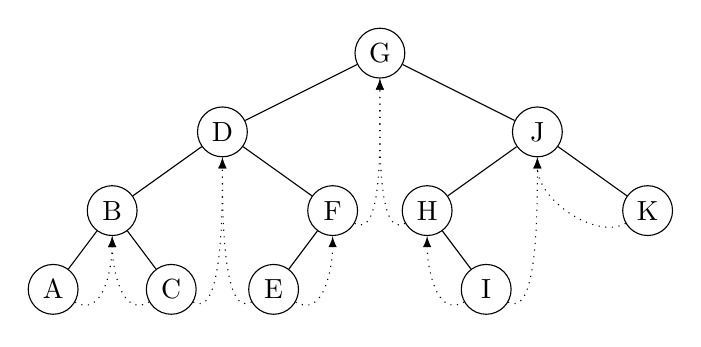
\begin{tikzpicture}
  \begin{scope}[
    level distance=10mm,
    every node/.style={draw,circle,inner sep=1pt,minimum size=1.8em},
    level 1/.style={sibling distance=40mm},
    level 2/.style={sibling distance=28mm},
    level 3/.style={sibling distance=15mm},
    ]
    \node(g){G}
    child{
      node(d){D}
      child{ node(b){B} child{ node(a){A} } child{ node(c){C} } }
      child{ node(f){F} child{ node(e){E} } child[missing] }
    }
    child{
      node(j){J}
      child{ node(h){H} child[missing] child{ node(i){I} } }
      child{ node(k){K} }
    };
  \end{scope}
  \begin{scope}[
    every path/.style={draw,dotted,>=latex},
    every to/.style={out distance=1.2em},
    left thread/.append style={out=210,in=270},
    right thread/.append style={out=330,in=270},
    ]
    \path[->] (a) to[right thread] (b);
    \path[->] (c) to[left thread] (b);
    \path[->] (c) to[right thread] (d);
    \path[->] (e) to[left thread] (d);
    \path[->] (e) to[right thread] (f);
    \path[->] (f) to[right thread] (g);
    \path[->] (h) to[left thread] (g);
    \path[->] (i) to[left thread] (h);
    \path[->] (i) to[right thread] (j);
    \path[->] (k) to[left thread] (j);
  \end{scope}
\end{tikzpicture}
\end{document}
